\chapter{Interferometria a retroiniezione}
\label{capitolo2}
\thispagestyle{empty}

\textit{In questo Capitolo verranno trattati i principi di base dell'interferometria, in particolare verrà presentata la tecnica utilizzata dello strumento di misura sviluppato in questo lavoro di Tesi: l'interferometria a retroiniezione. Dopo aver descritto il principio di funzionamento dell'interferometria a retroiniezione, saranno esposti i principali vantaggi, svantaggi e limitazioni di questa tecnica. In conclusione, verranno descritti i campi di applicazione della tecnica a retroiniezione ponendo particolare attenzione al campo d'applicazione dello strumento sviluppato: la misura di distanza assoluta.}

\section{Principi di interferometria convenzionale}
L'interferometria convenzionale è una tecnica che si basa sulla sovrapposizione di due o più fasci ottici, emessi dalla stessa sorgente, al fine di ottenere una frequenza di battimento (frequenza risultante dalla sovrapposizione) che contiene informazioni sui differenti cammini percorsi dai due fasci. Questa tecnica è in accordo con la teoria ondulatoria della luce che attribuisce alla propagazione della luce le caratteristiche della propagazione delle onde (elettromagnetiche) elastiche. Essa si basa sul fenomeno dell'interferenza e in particolare si sfrutta il principio secondo cui un'onda risultante dalla combinazione di due onde differenti mantiene proprietà che dipendono dalle onde generatrici.

I campi di applicazione di tale tecnica spaziano dall'astronomia alla metrologia ottica. Essa, in generale, trova applicazioni in ambiti dove l'ambiente di lavoro è critico (ad esempio superfici calde) o l'oggetto da misurare è difficilmente raggiungibile.
\begin{figure}  
  \begin{center}
    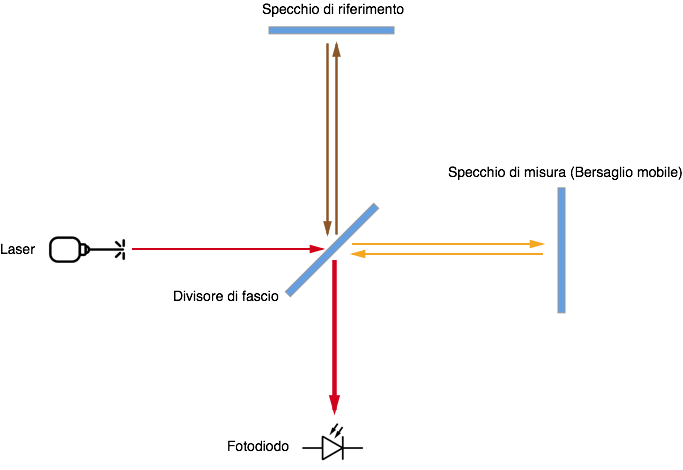
\includegraphics[scale=0.4]{cap2/michelson}
    \caption{Interferometro di \textit{Michelson}}
    \label{michelson}
  \end{center}
\end{figure}
La configurazione ottica interferometrica classica, mostrata in Figura \ref{michelson}, è definita interferometro di \textit{Michelson}~\cite{sensmeslaser}. Questa configurazione è costituita da una sorgente laser, un divisore di fascio (\textit{beam splitter}), due specchi e un fotodiodo.

Il funzionamento dell'interferometro di \textit{Michelson} consiste nel duplicare il fascio ottico emesso dalla sorgente laser, tramite uno specchio semiriflettente (divisore di fascio), in due cammini ottici distinti, di cui uno noto (di riferimento) e uno di misura. Entrambi i fasci, vengono riflessi da due specchi posti all'estremità dei due cammini. Lo specchio posto nel ramo di riferimento è fisso, mentre quello posto sul ramo di misura è mobile. Successivamente i fasci di riferimento e di misura vengono sovrapposti e indirizzati, attraverso il \textit{beam splitter}, verso il fotodiodo. Il fascio risultante è la combinazione di due fasci iso-frequenziali, ma sfasati a causa dei diversi cammini percorsi.

Infine, il fotodiodo produce una corrente, proporzionale all'intensitá del fascio laser incidente su di esso, che contiene l'informazione sullo spostamento del bersaglio. Tale corrente fotogenerata è associata alla potenza incidente che è proporzionale alla somma dei campi elettrici dei rispettivi cammini.

Indicando con ${E_m}$ il campo elettrico relativo al cammino di misura e con ${E_r}$ il campo elettrico relativo al cammino di riferimento, la corrente fotogenerata $I_{ph}$ segue la relazione:
\begin{equation}
\begin{split}
	I_{ph}&=\sigma|E_r+E_m|^2=\sigma|E_re^{i\phi_r}+E_me^{i\phi_m}|^2\\
	&=\sigma\{E_r^2+E_m^2+2E_rE_mRe[e^{i(\phi_m-\phi_r)}]\}\\
	&=I_r+I_m+2\sqrt{I_rI_m}\cos{(\phi_m-\phi_r)}
\end{split}
\end{equation}
dove $\sigma$ è il coefficiente di conversione del fotodiodo, $E_r$ e $E_m$ sono rappresentati come vettori rotanti di ampiezza $|E_{m,r}|$ e fase $\phi_{m,r}$ e la terza componente $2\sqrt{I_rI_m}\cos{(\phi_m-\phi_r)}$ costituisce la fase interferometrica. 

Per come é costruito l'interferometro di \textit{Michelson}, si avrà che la fase $\phi_r$ sará sempre costante, mentre quella relativa a $\phi_m$ varierá in funzione dello spostamento dell'ostacolo. Quindi ció che si ottiene sará una corrente fotogenerata che dipenderá dal coseno della fase $\phi_m$. 

Indicando con $k=\frac{2\pi}{\lambda}$ il numero d'onda (numero di oscillazione nell'unità di lunghezza) è possibile esplicitare l'argomento del coseno ottenendo:
\begin{equation}
	\phi=ks=\frac{2\pi}{\lambda}s	
\end{equation}
dove $\lambda$ è la lunghezza d'onda della sorgente laser e $s$ è lo spostamento.

Essendo $\phi_r= ks_r$ e $\phi_m = ks_m$, si può ricavare la variazione di fase totale, ottenendo:
\begin{equation}
	\Delta \phi=\phi_m-\phi_r=k(s_m-s_r)=\frac{2\pi}{\lambda}(s_m-s_r)
\end{equation}
dove $s_m$ e $s_r$ sono rispettivamente i cammini ottici di misura e di riferimento.

La variazione di fase del segnale interferometrico contiene quindi l'informazione sullo spostamento del bersaglio rispetto al cammino di riferimento. Il segnale interferometrico è quindi periodico per sfasamenti totali pari a $2\pi$, che corrispondono ad uno spostamento $s_m$ pari a $\frac{\lambda}{2}$. La misura avviene tramite il semplice conteggio delle frange interferometriche del segnale nel tempo. La risoluzione dello strumento di misura risulta quindi essere pari a  $\frac{\lambda}{2}$.

\subsection{Svantaggi dell'interferometria convenzionale} 
L'interferometro di \textit{Michelson} è molto vantaggioso dal punto di vista della semplicità di realizzazione perché vi è un impiego ridotto di componenti, ma presenta tuttavia notevoli svantaggi nella pratica:
\begin{figure}  
  \begin{center}
    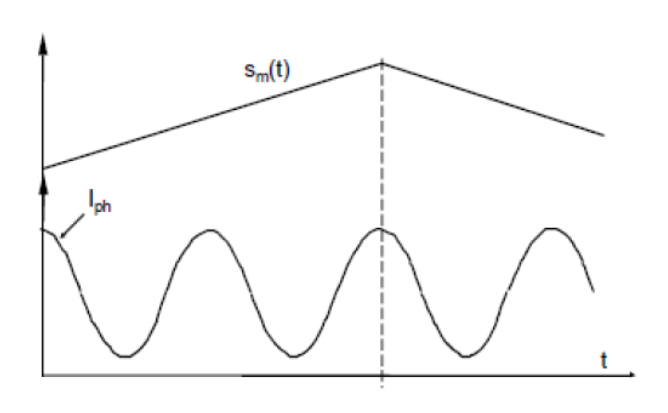
\includegraphics[scale=0.4]{cap2/versospost}
    \caption{Ambiguità sul verso di spostamento}
    \label{versospost}
  \end{center}
\end{figure}
\begin{itemize}
	\item L'allineamento degli specchi, per far convergere i due fasci di luce coerenti nello stesso punto, e il posizionamento del \textit{beam splitter} richiedono accuratezza elevata e sono quindi di difficile realizzazione.
	\item Richiede l'utilizzo di un bersaglio cooperativo e di una particolare ottica di collimazione. Non realizzabile in caso di misura non invasiva.
	\item Non permette di discriminare il verso di spostamento del bersaglio con conseguente ambiguità del movimento misurato. Tale ambiguità è causata dalla risposta cosinusoidale, come mostrato in Figura \ref{versospost}.
	\item La misura subisce alterazioni in caso di retroiniezione non voluta di luce esterna all'interno della cavità ottica del laser.
	\item L'utilizzo di sorgenti laser a gas comporta elevati costi di realizzazione dello strumento.
\end{itemize}
Tutto ciò ha fatto emergere la necessità di uno strumento che presentasse una semplicità di utilizzo e un costo contenuto.

\section{Interferometria a retroiniezione}
È stato esposto, nel paragrafo precedente, come l'interferometria convenzionale presenti notevoli svantaggi. Per tale motivo viene presentata una differente tecnica interferometrica: si tratta dell'interferometria a retroiniezione, chiamata anche interferometria a \textit{self-mixing}~\cite{1464-4258-4-6-371}.

La tecnica interferometrica a retroiniezione rende possibile la realizzazione di uno strumento di misura tramite il semplice utilizzo di una sorgente laser e di una lente per focalizzare il raggio ottico. Questa configurazione interferometrica risolve, quindi, i problemi dell'interferometria convenzionale, presentando una ridotta complessità di realizzazione e un costo contenuto. Per tale motivo il misuratore realizzato in questo lavoro di tesi sfrutta codesta tecnica.

\begin{figure}  
  \begin{center}
    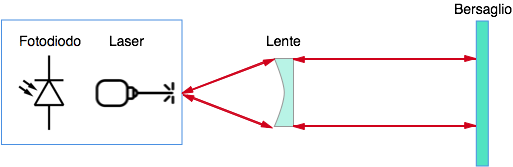
\includegraphics[scale=0.5]{cap2/selfmix}
    \caption{Schema di principio di un interferometro a retroiniezione}
    \label{selfmix}
  \end{center}
\end{figure}

La configurazione base del misuratore a \textit{self-mixing} è formata da un diodo laser, posto a distanza $s$ dal bersaglio, un'ottica collimatrice e un fotodiodo, che può essere anche quello di monitor integrato nello stesso package del laser. Lo schema base è riportato in Figura \ref{selfmix}.

La modalitá \textit{self-mixing}, a differenza dell'interferometro convenzionale, non utilizza porzioni di fascio ottico come riferimento. Per effettuare la misura viene sfruttata una porzione di luce riflessa dalla superficie del bersaglio che, rientrando nella cavità laser attraverso la lente, genera un battimento ottico con l'onda laser già presente. La luce riflessa dal bersaglio arriva con verso opposto al precedente cammino e con una potenza che è una frazione di quella emessa, a causa dell'attenuazione data dal tragitto laser-ostacolo-laser.

\'E possibile esplicitare la potenza della luce riflessa dal bersaglio con la relazione:
\begin{equation}
	P_r=\frac{P_0}{A}
\end{equation}
dove $P_0$ è la potenza ottica della radiazione emessa e $A$ è il coefficiente di attenuazione.

All'interno della cavità ottica del laser si verifica un fenomeno di interferenza: il campo elettrico $E_0$ della radiazione emessa si combina con il campo elettrico $E_r$ della luce retroiniettata. Come descritto nel paragrafo precedente, anche in questa situazione, $E_r$ risulta avere uno sfasamento ottico che è pari a:
\begin{equation}
	\phi=2ks
\end{equation}
dove $k=\frac{2\pi}{\lambda}$ è il numero d'onda e $s$ è la distanza.
\begin{figure}  
  \begin{center}
    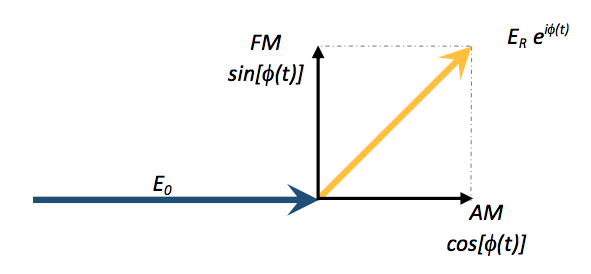
\includegraphics[scale=0.5]{cap2/rapprvet}
    \caption{Rappresentazione vettoriale dell'interferenza all'interno della cavità laser}
    \label{rapprvet}
  \end{center}
\end{figure}
Come mostrato in figura \ref{rapprvet} è possibile scomporre $E_r$, operando un'analisi vettoriale, nelle sue componenti in fase ed in ampiezza. Ciò permette, nella cavità ottica, sia la modulazione in frequenza (FM) che la modulazione in ampiezza (AM) del campo elettrico emesso originariamente dalla sorgente $E_0$. 

La componente che opera la modulazione d'ampiezza è $E_r\cos[\phi(t)]$, mentre la componente di modulazione di frequenza è $E_r\sin[\phi(t)]$. Le' due componenti sono sfasate di $90\degree$ e quindi la discriminazione dei due segnali in quadratura permette di ricavare senza ambiguità il verso dello spostamento del bersaglio, al contrario dell'interferometro di \textit{Michelson}.

L'equazione che governa la corrente nel fotodiodo sará:
\begin{equation}
	I_{ph}=I_0(1+m_{AM})\cos{[(1+m_{FM})\omega t]}
\end{equation}
dove $m_{AM}$ e $m_{FM}$ sono le profondità di modulazione.

Se si utilizza un laser a semiconduttore, come nel caso dello strumento presentato in questa Tesi, la componente FM presente nel fotodiodo é impossibile da estrarre in quanto presenta frequenze dell'ordine delle decine di $MHz$. Quindi, l'unica modulazione visibile sulla corrente del fotodiodo è quella AM:
\begin{equation}
	I_{ph}=I_0(1+m_{AM})\cos{[\omega t]}
\end{equation}
Il funzionamento di un diodo laser a singolo modo longitudinale soggetto a retroiniezione è descritto dalle equazioni differenziali sviluppate da Lang\&Kobayashi~\cite{1070479}; tuttavia, la risoluzione analitica di tali equazioni non è necessaria ai fini di questo lavoro di tesi.

Per questo motivo nel paragrafo successivo è presentata soltanto una soluzione qualitativa delle equazioni di Lang\&Kobayashi, con lo scopo di determinare i regimi di retroiniezione della tecnica \textit{self-mixing}.

\subsection{Regimi di retroiniezione tramite risoluzione qualitativa}
\begin{figure}  
  \begin{center}
    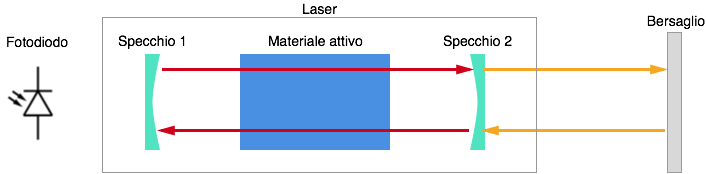
\includegraphics[scale=0.5]{cap2/roundtrips}
    \caption{Round trip ottico del campo elettrico all'interno della cavità laser}
    \label{roundtrips}
  \end{center}
\end{figure}
Un approccio qualitativo per determinare i regimi di retroiniezione è quello di considerare il \textit{round trip} del campo elettrico di Figura \ref{roundtrips}. In figura sono stati evidenziati i \textit{round trip} all'interno della cavità e tra il bersaglio e la cavità stessa.

Il campo elettrico totale presente all'interno della cavità è dato dalla somma di due campi elettrici: quello dovuto alla riflessione dello specchio interno posto al lato opposto della cavità e quello dovuto alla riflessione del bersaglio. Il campo elettrico risultante è quindi:
\begin{equation}
	E'=ER_1R_2e^{2\gamma L}e^{2jkL}+E\alpha e^{2jks}
\end{equation}
dove:
\begin{itemize}
	\item $R_1$ e $R_2$ sono rispettivamente le riflettività dello specchio in cavità e del bersaglio
	\item $\gamma$ è il guadagno netto per unità di lunghezza
	\item $L$ è la lunghezza della cavità
	\item $s$ è la distanza tra il secondo specchio ed il bersaglio
	\item $\alpha$ è il fattore di riflessione (o diffusione) del bersaglio
\end{itemize}

\'E possibile, quindi, ricavare facilmente dall'equazione precedente il guadagno d'anello:
\begin{equation}
	G_{loop}=\frac{E}{E'}=R_1R_2e^{2\gamma L}e^{2jkL}+\alpha e^{2jks}
	\label{gloop}
\end{equation}
Per far si che il sistema sia in grado di produrre oscillazioni spontanee che si mantengano nel tempo con ampiezza costante è necessario rispettare il criterio di \textit{Barkhausen}, il quale afferma che il sistema non deve modificare l'ampiezza del segnale e non deve introdurre sfasamento complessivo. Tali condizioni sono riassunte come segue:
\begin{equation}
	\begin{cases}
   |G_{loop}|=1\\\Phi_{loop} = 0
   \end{cases}
\end{equation}
Per studiare le soluzioni del sistema, si divide l'analisi del problema in due casi:
\begin{enumerate}
	\item In assenza di retroazione 
	\item In presenza di retroazione
\end{enumerate}
Nel primo caso, ovvero con coefficiente $\alpha$ nullo, si trovano le stesse equazioni di un normale laser in cui il guadagno e le perdite sono uguali, ovvero:
\begin{equation}
	\begin{cases}
   G_{loop}=R_1R_2e^{2\gamma L}\\\Phi_{loop} = 2kL=N2\pi
   \end{cases}
   \label{sistnoretr}
\end{equation}
con:
\begin{equation}
k=2\pi n_l \frac{\nu_0}{c}	
\end{equation}
\begin{equation}
	\nu_0 = N\frac{c}{2n_lL}
\end{equation}

dove $k$ è il numero d'onda, $\nu_0$ sono i modi di risonanza e $n_l$ rappresenta l'indice di rifrazione del mezzo attivo.

Se la frequenza reale si discosta da quella di risonanza propria, la frazione di fase $2kL$ in eccesso rispetto ad un multiplo di $2\pi$ può essere scritta come:
\begin{equation}
	2kL=4\pi n_l L \frac{\nu - \nu_0}{c}
\end{equation}

Infatti, in un interferometro con laser Fabry-Perot, la frequenza di risonanza diminuisce all'aumentare della lunghezza $L$ della cavità. Tale affermazione è resa valida dalla relazione differenziale:
\begin{equation}
	\frac{\Delta L}{L} = \frac{\Delta \lambda}{\lambda} = - \frac{\Delta \nu}{\nu}
\end{equation}

Se invece si è in presenza di retroiniezione (secondo caso), ovvero con coefficiente $\alpha$ non nullo, l'equazione \ref{gloop} diventa:
\begin{equation}
	R_1R_2e^{2\gamma L}\sin{ \left (4\pi n_l L \frac{\nu - \nu_0}{c} \right )} + \alpha \sin{(2ks)} = 0
	\label{regimeretr}
\end{equation}

Ipotizziamo il termine di variazione di frequenza $(\nu-\nu_0)$ abbastanza piccolo da poter approssimare $\sin(x)$ con $x$. Mettendo l'equazione \ref{regimeretr} a sistema con le equazioni presenti in \ref{sistnoretr} e considerando l'approssimazione e la sostituzione dei parametri, si ottiene la condizione di risonanza:
\begin{equation}
	2ks=4\pi s \frac{\nu}{c} \approx 4\pi s \frac{\nu_0}{c}
\end{equation}
\begin{equation}
	(\nu - \nu_0) + \left[ \frac{c}{4\pi n_l L}\alpha \sin{\left (\frac{4 \pi s \nu_0}{c}\right )} \right] = 0
\end{equation}

Indicando, infine, con $\nu'=(\nu-\nu_0)$ lo scostamento della frequenza reale rispetto a quella ideale, la modulazione della frequenza vale: 
\begin{equation}
	\nu'= \frac{c}{4\pi n_l L} \alpha \sin \left ( \frac{4 \pi s \nu_0}{c} \right )
\end{equation}

\begin{figure}  
  \begin{center}
    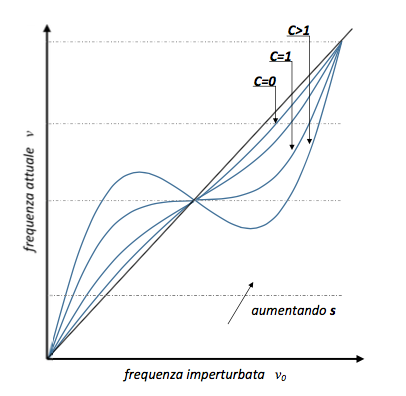
\includegraphics[scale=0.5]{cap2/pertfreq}
    \caption{Perturbazione della frequenza reale rispetto alla frequenza ideale}
    \label{pertfreq}
  \end{center}
\end{figure}

In Figura \ref{pertfreq} è rappresentata la relazione tra la frequenza reale $\nu$ e la frequenza imperturbata $\nu_0$ all'aumentare dello spostamento $s$ del bersaglio. Dalla relazione si ottiene una sinusoide sovrapposta alla bisettrice del primo quadrante periodica di $2\pi$. 

Ogni salto è equivalente a spostamenti $s$ pari a $\frac{\lambda}{2}$, quindi la distanza del bersaglio si puó esprimere come un multiplo intero di $\frac{\lambda}{2}$ sommato allo scarto $\Delta s$:
\begin{equation}
	s= N \frac{\lambda}{2} + \Delta s
\end{equation}
assumendo $\Delta s$ minore di $\frac{\lambda}{2}$.

Le intersezioni tra le linee tratteggiate e le curve sinusoidali, mostrate in Figura \ref{pertfreq}, indicano i punti di lavoro del sistema: spostando il bersaglio della quantità $\delta s$, la frequenza reale assume il valore dato dall'intersezione tra la linea tratteggiata e la curva.

In base all'ampiezza della sinusoide si possono distinguere due regimi di funzionamento:
\begin{enumerate}
	\item \textit{Regime di bassa retroiniezione}
	\item \textit{Regime di alta retroiniezione}
\end{enumerate}

Si dice regime di bassa iniezione quando l'ampiezza della sinusoide sovrapposta è piccola e vi è un unico punto di intersezione che corrisponde alla frequenza reale $\nu$.

Si dice regime di alta iniezione, invece, quando l'ampiezza della sinusoide è grande e vi sono tre o più punti di intersezione rappresentanti la frequenza reale $\nu$. Per distinguere la frequenza effettiva, in regime di alta iniezione, è necessario conoscere le condizioni del laser prima dello spostamento $\Delta s$~\cite{randonethesis}.

Il limite tra i due regimi sta nel punto centrale del grafico in cui vi è un flesso a tangente orizzontale. Tale condizione può essere espressa matematicamente con il sistema:
\begin{equation}
	\begin{cases}
   \frac{d(y=x+Asin(Bx))}{dx}=0\\Bx=\pi
   \end{cases}
   \label{sistflesso}
\end{equation}
dove $A=- \frac{c}{4 \pi n_l L}\alpha$ e $B=\frac{4\pi s}{c}$. Dal sistema \ref{sistflesso} si ricava $AB=1$ e sostituendo i parametri fisici si ottiene:
\begin{equation}
	\frac{c}{4 \pi n_l L} \alpha \frac{4\pi s}{c} = \frac{\alpha s}{n_l L} = 1
\end{equation}

Arrivati a questo punto si è in grado di definire il fattore $C$ come indice della retroiniezione del sistema interferometrico a \textit{self-mixing}:
\begin{equation}
	C = \frac{\alpha s}{n_l L}
\end{equation}

Nel caso in cui la sorgente laser considerata utilizzi come materiale attivo un semiconduttore, il parametro $C$ diventa:
\begin{equation}
	C=\alpha s \frac{\sqrt{1+\alpha_{en}^2}}{n_l L}
\end{equation}
dove $\alpha_{en}$ è il fattore di allargamento di riga che tipicamente assume valori tra $2$ e $6$ nel caso di laser a stato solido.

Come descritto in precedenza non verrà trattata la risoluzione matematica delle equazioni di Lang\&Kobayashi, ma si analizzeranno solo i risultati. Per una trattazione completa si faccia riferimento alla letteratura~\cite{1070479}.

Risolvendo le equazioni di Lang\&Kobayashi si ottiene che con lo spostamento del bersaglio, non è modulata unicamente la frequenza propria di oscillazione del laser, ma anche la potenza ottica emessa dal laser, che in condizioni di retroazione è pari a:
\begin{equation}
	P(\Phi)=P_0(1+mF(\Phi))
\end{equation}
dove:
\begin{itemize}
	\item $P_0$ è la potenza emessa del laser in assenza di retroiniezione 
	\item $m$ rappresenta l'ampiezza del segnale a frange sovrapposto al termine costante (profondità di modulazione)
	\item $\Phi = 2ks$ è lo sfasamento tra l'onda emessa e quella retroiniettata 
	\item $F(\Phi)$ è una funzione di periodo $2\pi$ che assume valori di ampiezza compresi tra $-1$ e $+1$:
		\begin{equation}
			F(\Phi(t))=F(2ks(t))=F(2\frac{2\pi}{\lambda}s(t))
		\end{equation}
\end{itemize}

L'andamento della funzione $F(\Phi)$ è influenzato dal fattore $C$. La conseguenza è che $F(\Phi)$  dipende da 3 fattori:
\begin{enumerate}
	\item distanza del bersaglio
	\item riflettività del bersaglio 
	\item parametri del laser
\end{enumerate}
Si possono, quindi, identificare quattro possibili regimi di funzionamento per un interferometro a \textit{self-mixing} sulla base del parametro $C$:
\begin{enumerate}
	\item \textit{Regime di retroiniezione molto debole} ($0 < C \leq 0.1$): la quantità di potenza ottica che rientra in cavità è molto ridotta a causa di un'elevata riflettività degli specchi o di bassi coefficienti di riflessione della superficie del bersaglio. La funzione $F(\Phi)$ è un coseno di ampiezza molto ridotta, tipicamente $10^{-4}$ rispetto al valore in continua.
	\item \textit{Regime di retroiniezione debole} ($0.1 < C < 1$): La funzione $F(\Phi)$ inizia a distorcersi e non è più simmetrica. La maggior parte dei casi pratici rientra in questo regime di funzionamento. 
	\item \textit{Regime di retroiniezione moderata} ($1 < C \leq 4.6$): Per i valori di $C$ presenti in questo intervallo ci sono tre punti di intersezione in Figura \ref{pertfreq}, che indicano bruschi salti di potenza ottica.
	\item \textit{Regime di retroiniezione forte} ($C>4.6$): Avviene quando la luce retroiniettata in cavità è al massimo pari a quella incidente, nel quale ci sono cinque o più punti di equilibrio.
\end{enumerate}
\begin{figure}  
  \begin{center}
    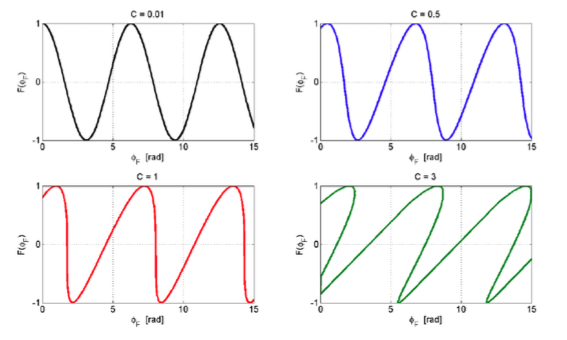
\includegraphics[scale=0.5]{cap2/regimifunz}
    \caption{Regimi di retroiniezione: funzione $F(\Phi)$ al variare del parametro $C$}
    \label{regimifunz}
  \end{center}
\end{figure}
\begin{figure}  
  \begin{center}
    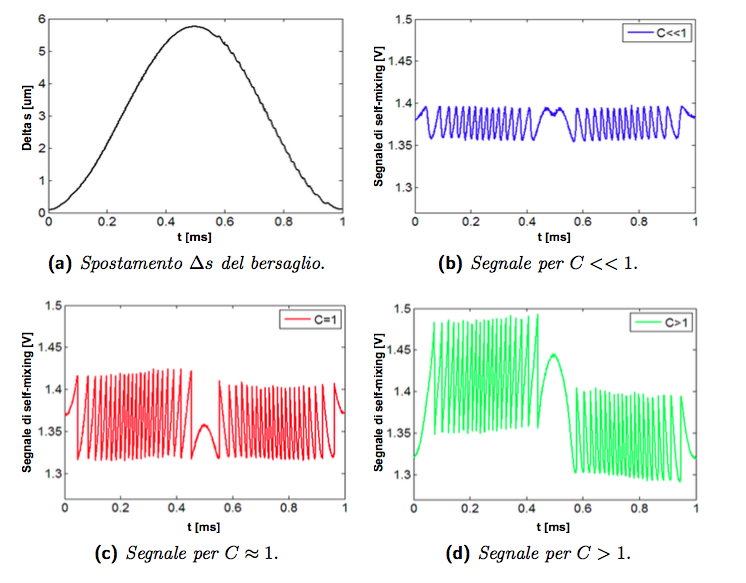
\includegraphics[scale=0.4]{cap2/regimisegn}
    \caption{Esempi di segnale interferometrico per i differenti valori del parametro $C$}
    \label{regimisegn}
  \end{center}
\end{figure}
In Figura \ref{regimifunz} è mostrata la forma della funzione $F(\Phi)$ nei 4 possibili regimi di funzionamento. Nella Figura \ref{regimisegn} è mostrato, invece, il segnale di comando del bersaglio e i rispettivi segnali interferometrici a frange al variare del parametro $C$.

Il segnale risultante è periodico in $\Phi$ e mostra le tipiche frange interferometriche ogni volta che la fase varia di $2\pi$. Ciascuna frangia corrisponde ad uno spostamento $\frac{\lambda}{2}$ del bersaglio~\cite{341714}.

\subsection{Vantaggi e svantaggi dell'interferometria a retroiniezione}
La tecnica \textit{self-mixing} ha diversi vantaggi rispetto agli strumenti basati su altri principi, come i telemetri visti nel Capitolo precedente.

I principali vantaggi sono:
\begin{itemize}
	\item \underline{Semplicità strutturale}: Il sistema interferometrico non necessita dell'uso di un canale ottico di riferimento o di divisori di fascio. L'informazione dello spostamento è ricavata direttamente dalla potenza emessa dal laser.
	\item \underline{Semplicità di rilevamento}: Il rilevamento si basa sull'osservazione della distorsione delle frange, più semplice del rilevamento nell'interferometro di \textit{Michelson}. Inoltre, l'allineamento ottico del bersaglio non è particolarmente critico ed è possibile eseguire misure valide su molteplici tipologie di superficie del bersaglio.
	\item \underline{Performante}: La semplicità di rilevamento permette di ottenere uno strumento di misura performante.
	\item \underline{Non ambiguità del verso dello spostamento}: Il problema dell'ambiguità del verso di spostamento non è presente perché tale informazione è intrinseca nella forma d'onda $F(\Phi)$. Per tale motivo non si rende necessario l'utilizzo di un secondo canale di misura interferometrico. 
	\item \underline{Elevata sensibilità}: Si basa su un sistema ottico coerente che estrae le informazioni dalla sorgente di luce, a differenza della tecnica di triangolazione.
\end{itemize}
Tuttavia, l'interferometria a retroiniezione presenta anche diversi svantaggi:
\begin{itemize}
	\item \underline{Salti di modo}: Sono dovuti a variazioni di corrente o di temperatura nei laser a semiconduttore. Essi influenzano negativamente la misura dell'interferometro, degradandone le prestazioni.
	\item \underline{Dipendenza della misura da variabili esterne}: Variabili esterne come temperatura e pompaggio di corrente incidono sulla lunghezza d'onda d'emissione del laser, grandezza dalla quale dipende direttamente la misura, causando una ridotta accuratezza della misura.
	\item \underline{Decadimento della luce coerente}: \'E possibile che la potenza retroiniettata passi a regimi di alta iniezione compromettendo le misure o, in casi limite, danneggiando irreparabilmente il laser. 
\end{itemize}

\section{Principali limitazioni della tecnica interferometrica}
Indipendentemente dalla configurazione di interferometro scelta, le prestazioni della tecnica intereferometrica presentano limiti dovuti a molteplici cause. Le principali sono descritte di seguito.
\begin{figure}  
  \begin{center}
    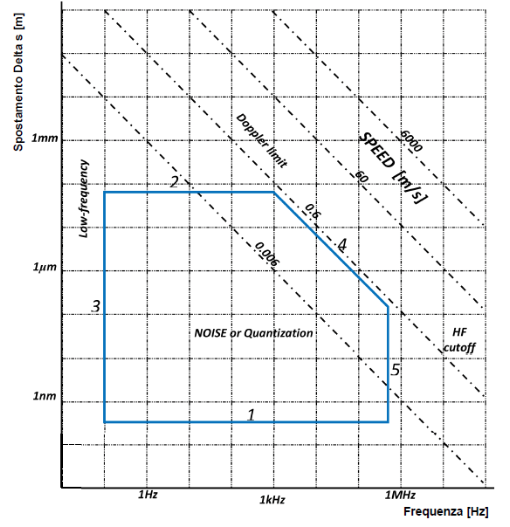
\includegraphics[scale=0.4]{cap2/wegel}
    \caption{Diagramma di Wegel}
    \label{wegel}
  \end{center}
\end{figure}
\begin{figure}  
  \begin{center}
    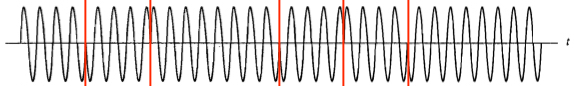
\includegraphics[scale=0.4]{cap2/saltifase}
    \caption{Esempio di salti di fase dell'onda nel tempo}
    \label{saltifase}
  \end{center}
\end{figure}
\begin{figure}  
  \begin{center}
    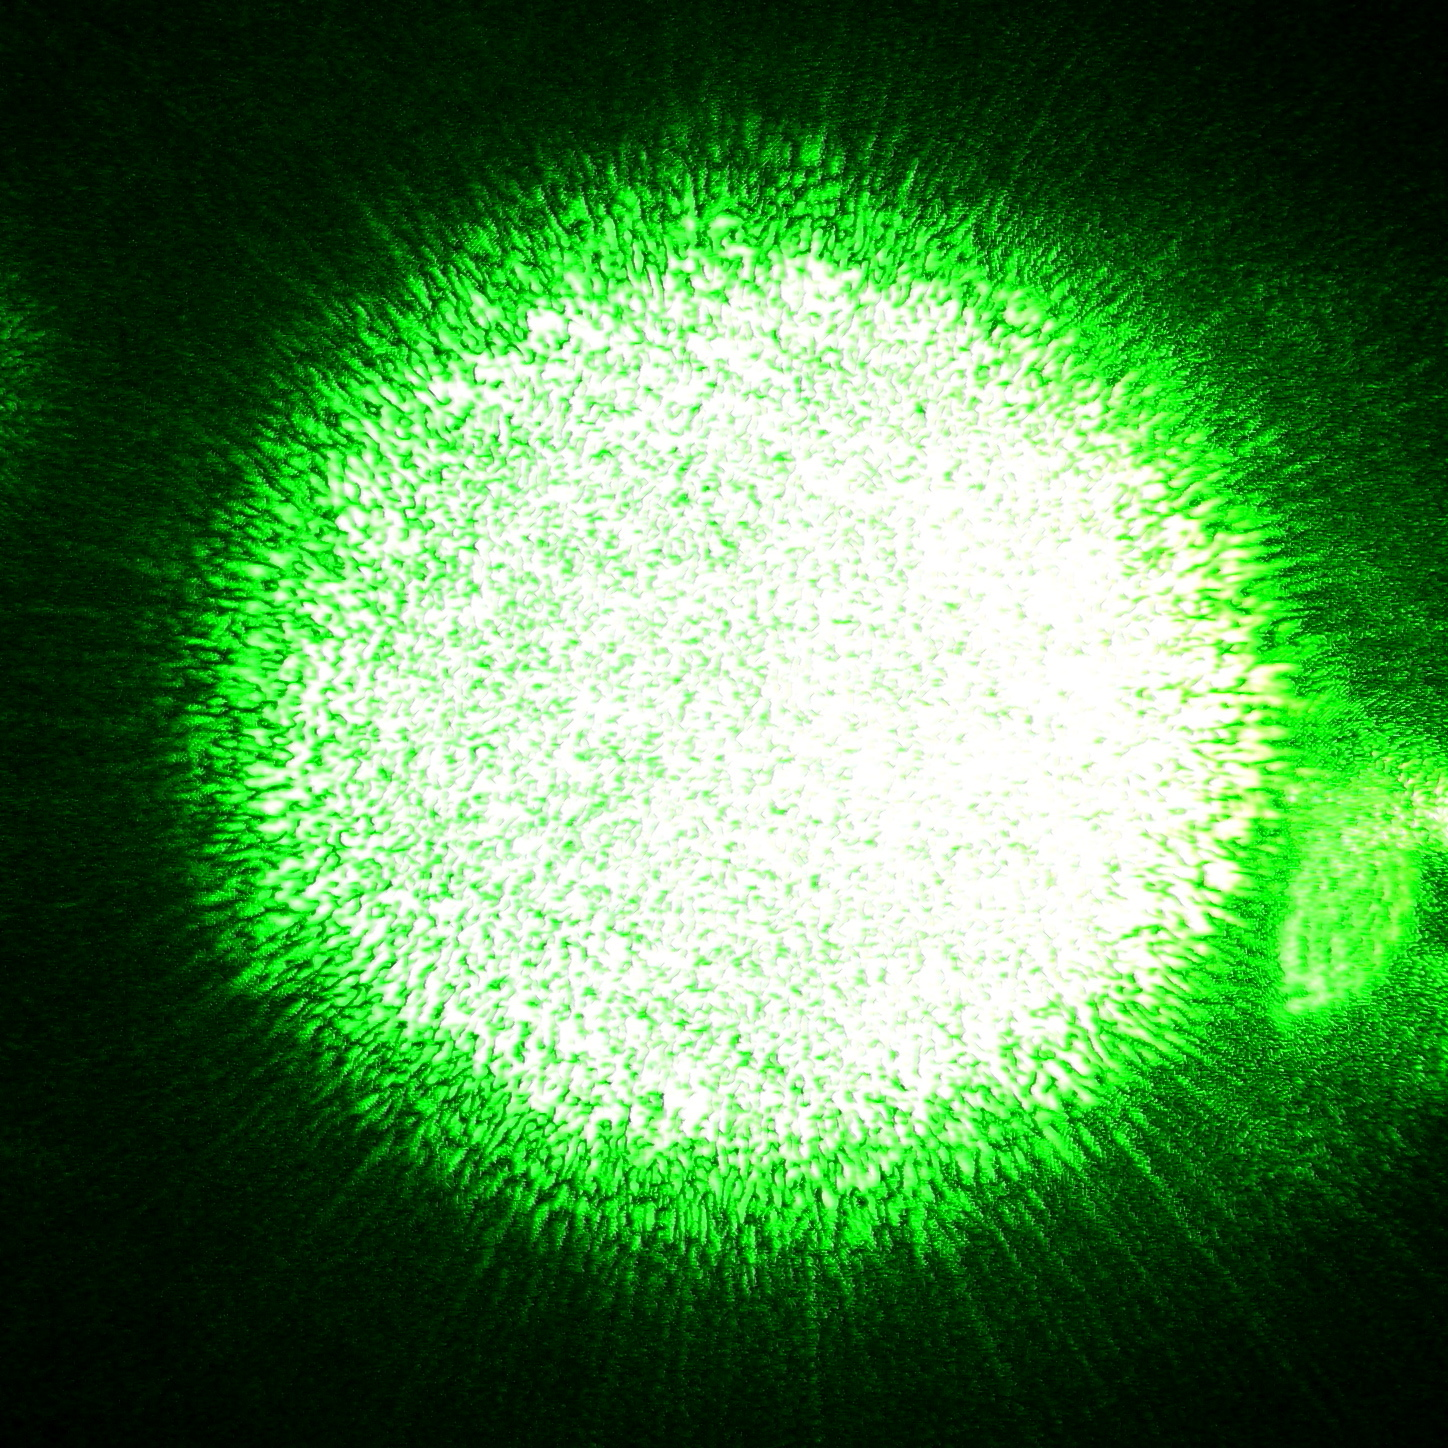
\includegraphics[scale=0.1]{cap2/spackle}
    \caption{Speckle causato da una superficie diffusiva}
    \label{spackle}
  \end{center}
\end{figure}
\begin{itemize}
	\item \underline{Limitazioni nel piano spostamento-frequenza}: Il diagramma di Wegel, rappresentato in Figura \ref{wegel}, è utilizzato per analizzare la qualità di un interferometro in termini di prestazioni e limiti. Il diagramma presenta 5 segmenti che delimitano un'area chiamata "zona di funzionamento". Maggiore sarà l'area della zona di funzionamento maggiore risulterà il campo d'azione dello strumento di misura.
 
		I 5 segmenti rappresentano, in particolare, 5 limitazioni qui di seguito riportate:
		\begin{itemize}
		\item \textit{Minimo spostamento misurabile}: Il segmento inferiore 1 definisce la sensibilità dello strumento al minimo spostamento misurabile in base al rumore elettronico di fondo.
		\item \textit{Massimo spostamento misurabile}: Il segmento superiore 2 impone il limite massimo di spostamento del bersaglio affinché lo strumento funzioni correttamente.
		\item \textit{Frequenza minima dello spostamento}: Il segmento laterale sinistro 3 indica la minima frequenza di vibrazione in accordo con la minima banda di segnale dell'elettronica di elaborazione.
		\item \textit{Frequenza massima dello spostamento}: Il segmento laterale destro 5 indica la massima frequenza di vibrazione in accordo con la massima banda di segnale dell'elettronica di elaborazione.
		\item \textit{Velocità di spostamento massima}: Il segmento obliquo 4 mostra la velocità limite di spostamento massimo, che è proporzionale al prodotto tra la frequenza di oscillazione e la sua ampiezza.
		\end{itemize}
	
	\item \underline{Coerenza temporale}: Un qualunque fascio coerente generato da un laser ha una lunghezza di coerenza limitata, ovvero dopo un certo tempo dalla sua emissione la fase dell'onda cambia ed assume un valore casuale. Dunque il campo emesso da un laser presenta salti di fase a intervalli casuali, come mostrato in Figura \ref{saltifase}. Indicando con $T_{coh}$ la coerenza temporale e con $L_{coh}$ la lunghezza di coerenza, è possibile scrivere:
		\begin{equation}
			\begin{cases}
				L_{coh}=cT_{coh}\\T_{coh}=\frac{1}{\Delta \nu}
			\end{cases}
		\end{equation}
		dove $c$ è la velocità della luce nel vuoto e $\Delta \nu$ è la larghezza di riga in frequenza.
		
		Dalle precedenti relazioni è possibile ricavare la distanza massima dell'ostacolo affinché non si perda la proprietà di coerenza:
		\begin{equation}
			s_{max}=|s_m - s_r|_{max}=\frac{c}{\Delta \nu} = L_{coh}
		\end{equation}
		Se la distanza dell'ostacolo è maggiore di $L_{coh}$ non si ha segnale interferometrico ma solo rumore dunque non è possibile effettuare misure valide non potendo contare correttamente le frange interferometriche. Questo rumore è definito come rumore di fase. Solitamente il rumore di fase è il contributo dominante nella determinazione del minimo spostamento misurabile. 
		
		Tuttavia esiste un altro contributo che limita le prestazioni: il rumore quantico. Tale rumore risulta essere quasi sempre trascurabile perché il rumore di fase è dominante rispetto ad esso.
		\item \underline{Speckle-Pattern}: \'E un fenomeno dovuto alla superficie del bersaglio. In particolare, se un fascio di luce coerente colpisce un bersaglio avente superficie diffondente la luce retrodiffusa avrà una distribuzione di potenza granulare e non omogenea. Il fenomeno è mostrato in Figura \ref{spackle}.
		
			La luce retrodiffusa è generata dalla combinazione di due fasci di luce: una porzione di fascio riflessa in modo speculare alla direzione di incidenza e l'altra porzione di fascio diffusa uniformemente nello spazio. Quest'ultima è causata da imperfezioni superficiali del bersaglio.
			
			Ogni imperfezione superficiale, chiamata avvallamento, si comporta come un diffusore di luce secondario debolmente correlato ad un avvallamento adiacente. Il campo risultante, in un punto $P$ difronte alla superficie dell'ostacolo, è formato dalla sovrapposizione delle onde generate da ciascun avvallamento.
			
			 L'effetto di tale sovrapposizione è il risultato dell'interferenza costruttiva e distruttiva di onde aventi fase diversa. Ogni granulo ottico così formato prende il nome di \textit{speckle}. Geometricamente si definisce \textit{speckle} un ellissoide avente variazioni di fase contenute nel $50\%$ e dimensioni trasversali ($S_t$) e longitudinali ($S_l$) pari a:
			 \begin{equation}
			 	S_t=\lambda \left ( \frac{z_0}{D} \right )^2
			 \end{equation}
			 \begin{equation}
			 	S_l=\lambda \left ( 2 \frac{z_0}{D} \right )^2
			 \end{equation}
			 dove $z_0$ è la distanza tra il punto di osservazione e il bersaglio e $D$ è la dimensione di macchia su di esso.
			 
			 Nelle misure basate sulla tecnica di interferometria a retroiniezione, lo \textit{speckle-pattern} rappresenta il fattore limitante più grande. A causa di tale disturbo, il segnale interferometrico risulterà interrotto ogni qual volta che il fascio di luce incontrerà uno \textit{speckle}. \'E possibile limitare questa problematica aumentando la potenza ottica retro-iniettata o adottando il sistema ottico più adatto per l'applicazione in questione.
	\item \underline{Dispersione del mezzo}: Il fascio ottico che si propaga fuori cavità subisce delle alterazioni dovute alle caratteristiche di ogni mezzo che esso attraversa, che ne modifica la lunghezza d'onda. I fattori che incidono maggiormente sono temperatura e pressione del mezzo. Per minimizzare il contributo dispersivo di questi fattori vengono impiegati stabilizzatori di temperatura e pressione ambientale.
\end{itemize}

\begin{figure}  
  \begin{center}
    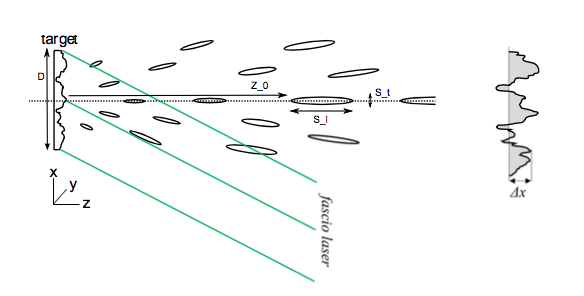
\includegraphics[scale=0.5]{cap2/specklegeom}
    \caption{Rappresentazione esemplificata del fenomeno dello speckle-pattern}
    \label{specklegeom}
  \end{center}
\end{figure}

\section{Applicazioni dell'interferometria a retroiniezione}
La tecnica interferometrica a retroiniezione può essere utilizzata in quattro principali campi di applicazione:
\begin{itemize}
	\item \underline{Misura di distanza assoluta}: Tecnica per la misurazione di distanza tra lo strumento di misura e un oggetto remoto (bersaglio).
	\item \underline{Velocimetria}: Tecnica per la misurazione di velocità a distanza.
	\item \underline{Vibrometria}: Tecnica per la misurazione delle vibrazioni. Il vibrometro laser è utile quando non è possibile installare un accelerometro sull'oggetto da misurare. Si basa sul principio di aggancio di fase~\cite{thesismelch}.
	\item \underline{Misura di spostamenti}: Tecnica per la misurazione dello spostamento di un bersaglio. Si basa sul conteggio delle frange interferometriche di periodicità $\frac{\lambda}{2}$ al variare della distanza dal bersaglio.
\end{itemize}

La misura di distanza assoluta, oggetto del seguente lavoro di Tesi, verrà discussa ampiamente nel paragrafo successivo.

\subsection{Misura di distanza assoluta}
Come descritto in precedenza, un segnale interferometrico è caratterizzato dalla seguente relazione:
\begin{equation}
	\phi = 2ks = 2 \frac{2\pi}{\lambda}s
	\label{distass}
\end{equation}
che rappresenta lo sfasamento del campo elettrico retroiniettato rispetto al campo elettrico emesso.

Da tale relazione si nota che per generare un segnale interferometrico è necessario uno spostamento $s$ del bersaglio o una variazione della lunghezza d'onda $\lambda$ del fascio emesso dal laser. Considerando come campo di applicazione la misura di distanza assoluta è necessario agire solo sulla lunghezza d'onda $\lambda$ e non sullo spostamento $s$ dato che il bersaglio è immobile.

Un metodo per variare la lunghezza d'onda $\lambda$ è quello di modulare la corrente di pompa della sorgente laser:
\begin{equation}
		\lambda_{new}=\lambda_{old}+\chi\Delta I
		\label{lungondanew}
\end{equation}
dove $\chi$ è la variazione di lunghezza d'onda rispetto alla variazione di corrente. La variazione di lunghezza d'onda $\chi$ è pari a $\chi = \frac{\Delta \lambda}{\Delta I}$ ed è espressa in $\left [ \frac{pm}{mA} \right ]$. Tale parametro varia molto da dispositivo a dispositivo. Esso risulta, inoltre, fortemente non lineare in alcune zone di funzionamento della sorgente laser. 

Differenziando l'equazione \ref{lungondanew}, rispetto alla lunghezza d'onda $\lambda$, è possibile ottenere la variazione di fase del segnale interferometrico:
\begin{equation}
	\frac{d\phi}{d\lambda}=-2\frac{2\pi}{\lambda^2}s
\end{equation}
da cui si può ricavare la misura di distanza assoluta $s$:
\begin{equation}
	s=-\frac{d\phi}{d\lambda}\frac{\lambda^2}{4\pi}
\end{equation}
Infine, la misura di distanza assoluta s può essere compiuta in due modi:
\begin{enumerate}
	\item \underline{Conteggio del numero di frange}: Questo metodo consiste nel contare il numero di frange visibili nel segnale interferometrico. Il numero di frange ad una distanza fissata $s$ dipende dalla variazione della lunghezza d'onda. Nota la variazione della lunghezza d'onda, più precisamente il periodo in cui viene fornita la variazione di corrente che genera la variazione di lunghezza d'onda, è possibile misurare la distanza assoluta del bersaglio con la seguente equazione:
	\begin{equation}
		s=\frac{N_F}{\Delta \lambda}\frac{\lambda^2}{2}
	\end{equation}
	dove $N_F$ rappresenta il numero di frange pari a:
	\begin{equation}
		N_F=\frac{\Delta \phi}{2 \pi}
	\end{equation}
	Questo metodo ha una scarsa accuratezza poiché la risoluzione massima ottenibile è data dalla singola frangia. 
	\item \underline{Misura del tempo di frangia}: Questo metodo consiste nella misura del periodo di frangia. Definendo con $t_{frangia}$ la lunghezza del periodo di frangia, è possibile scrivere la seguente proporzione:
	\begin{equation}
		\Delta \lambda_{2\pi} : \Delta \lambda = t_{frangia} : \Delta t
	\end{equation}
	dove $\Delta \lambda_{2\pi}$ è la variazione di lunghezza d'onda 
che produce una variazione di fase interferometrica $\Delta \phi$ pari a $2\pi$.
	
	Dalla precedente relazione è possibile ricavare la variazione di lunghezza d'onda $\Delta \lambda_{2\pi}$:
	\begin{equation}
		\Delta \lambda_{2\pi} = \frac{t_{frangia}}{\Delta t} \Delta \lambda = \frac{\Delta \lambda}{\Delta I}\frac{\Delta I}{\Delta t} t_{frangia}
	\end{equation}
	Per ricavare la distanza assoluta $s$ è necessario fare riferimento alla relazione:
	\begin{equation}
		\left ( 2\frac{2\pi}{\lambda}-2\frac{2\pi}{\lambda + \Delta \lambda_{2\pi}} \right ) s = 2\pi
	\end{equation}
	che eguaglia la differenza di fase causata da una variazione di lunghezza d'onda $\Delta \lambda_{2\pi}$ a $2\pi$.
	
	Infine, per ricavare la distanza $s$, è necessario approssimare $(\lambda + \Delta \lambda_{2\pi}) \approx \lambda$ poiché $\lambda \gg \Delta \lambda_{2\pi}$:
	\begin{equation}
		s \approx \frac{\lambda^2}{2\frac{\Delta \lambda}{\Delta I}\frac{\Delta I}{\Delta t} t_{frangia}} =  \frac{\lambda^2}{2\frac{\Delta \lambda}{\Delta I}\frac{\Delta I}{\Delta t}}f_{frangia}
	\end{equation}
	dove $f_{frangia}=\frac{1}{t_{frangia}}$ è il tono fondamentale del segnale interferometrico.
	
	Lo strumento di misura descritto in questo elaborato, deve essere in grado di effettuare la misura anche con ostacolo in movimento. Per tale motivo occorre scegliere un'opportuna forma d'onda per realizzare la modulazione in corrente.
	
	Come già detto in precedenza, uno spostamento dell'ostacolo provoca una variazione di fase del segnale interferometrico. Richiamando che la variazione di fase causata dalla modulazione equivale a:
	\begin{equation}
		\frac{d\phi_{mod}}{dt} = 2 \pi f_{mod}
	\end{equation}
	e derivando la relazione \ref{distass} rispetto allo spazio:
	\begin{equation}
		\frac{d\phi_s}{ds}=2\frac{2\pi}{\lambda}
	\end{equation}
	è possibile ottenere:
	\begin{equation}
		\frac{d\phi_s}{ds}=2\pi f_s
	\end{equation}
	dove $f_s$ è la frequenza media delle frange prodotte a causa dello spostamento.
	
	Da questo si deduce che: se il bersaglio è in movimento la variazione di fase complessiva del segnale interferometrico è data dalla somma di due componenti: $\phi_{mod}$ e $\phi_s$.
	Per compensare il contributo indesiderato $\phi_s$ è necessario realizzare una modulazione di corrente che vada a incrementare e decrementare la lunghezza d'onda della sorgente laser. Per fare ciò, si utilizza un segnale a forma triangolare con ampiezza opportuna.
	
	Un accorgimento atto a compensare e minimizzare gli sfasamenti consiste nell'esecuzione, durante il processo di misura, di una media tra il periodo di frangia valutato nella fase ascendente e il periodo di frangia valutato nella fase discendente della triangolare di modulazione allo scopo di aumentare la sensibilità dello strumento rispetto allo spostamento. 
	
Da questa osservazione si ottiene la relazione:
\begin{equation}
	s \propto \frac{f_{rise}+f_{fall}}{2} = \frac{ \left | \frac{d\phi_{rise}}{dt} + \frac{d\phi_{fall}}{dt} \right |}{2}
	\label{eqrisefall}
\end{equation}
dove $f_{rise}$ e $f_{fall}$ sono rispettivamente il tono fondamentale del segnale interferometrico nella rampa di salita e discesa dell'onda triangolare.

Sapendo che la fase complessiva del segnale interferometrico è formata dai due contributi discussi in precedenza è possibile sostituire nella relazione \ref{eqrisefall} la fase totale $\phi_{tot} = \phi_{mod} + \phi_s$:
\begin{equation}
	s \propto \frac{ \left | \frac{d\phi_{mod}}{dt} + \frac{d\phi_{s}}{dt} \right |+ \left | \frac{d\phi_{mod}}{dt} - \frac{d\phi_{s}}{dt} \right |}{2} = \frac{d\phi_{mod}}{dt}
\end{equation}
Infine, in questo modo è possibile misurare la distanza assoluta eliminando così il contributo indesiderato $\phi_s$ causato da un eventuale spostamento del bersaglio.

Esprimendo le grandezze $f_{rise}$ e $f_{fall}$ attraverso le seguenti relazioni:
\begin{equation}
	f_{rise}= \left | \frac{1}{2\pi} \frac{\delta \phi}{\delta t} \right | = \left | - \frac{2s}{\lambda^2} \frac{\delta \lambda}{\delta t} + \frac{2}{\lambda} \frac{\delta s}{\delta t} \right | = \left | - \frac{2sk}{\lambda^2} \frac{\Delta I}{\Delta T} + \frac{2}{\lambda}v \right |
\end{equation}
\begin{equation}
	f_{fall}= \left | \frac{1}{2\pi} \frac{\delta \phi}{\delta t} \right | = \left | \frac{2s}{\lambda^2} \frac{\delta \lambda}{\delta t} + \frac{2}{\lambda} \frac{\delta s}{\delta t} \right | = \left | \frac{2sk}{\lambda^2} \frac{\Delta I}{\Delta T} + \frac{2}{\lambda}v \right |
\end{equation}
dove $v$ è la velocità del bersaglio e $T$ è il semiperiodo della triangolare di modulazione, è possibile definire l'equazione della distanza assoluta $s$ in maniera più precisa:
\begin{equation}
	s = \frac{f_{rise}+f_{fall}}{2} \left [ \frac{\lambda^2}{2k\left ( \frac{\Delta I}{\Delta T} \right )}  \right ]
\end{equation}
Questa tecnica risulta più accurata della precedente perché è limitata solamente dalla precisione con la quale è possibile misurare il periodo e dalla capacità della sorgente di generare un segnale interferometrico ripetibile. 

\end{enumerate}

%%TODO Cap 2: Controllare le formule